\chapter{Resultados}

\subsection{Metricas globales del detector}

La tabla~\ref{tab:metricas} resume el rendimiento de los tres
detectores sobre el bloque de test (15\% final de los datos
simulados, split temporal por bloques). Los valores provienen del
prototipo ejecutable incluido en este trabajo (notebook
\texttt{gemelo\_digital\_se\_ejecutado.ipynb}, semilla 42, CPU).

\begin{table}[ht]
\centering
\small
\caption{Comparacion de detectores sobre el bloque de test (prototipo ejecutable).}
\label{tab:metricas}
\begin{tabular}{lrrrrl}
\toprule
\textbf{Detector} & \textbf{FPR} & \textbf{TPR} & \textbf{F1} & \textbf{AUC} & \textbf{Privacidad} \\
\midrule
Estatico 3-sigma            & 12.8\% & 36.8\% & 0.42 & 0.639 & no \\
AE-LSTM centralizado        &  4.9\% & 76.3\% & 0.80 & 0.878 & no (centralizado) \\
AE-LSTM federado (3 SEs)    &  5.0\% & 80.5\% & 0.87 & 0.906 & si (datos en origen) \\
\bottomrule
\end{tabular}
\end{table}

\subsubsection{Lectura de los resultados}

El prototipo alcanza el rango proyectado por la literatura (FPR
$\approx$ 5\%, TPR $\approx$ 75-85\%) sin escalar modelo ni datos:
con \texttt{hidden=32}, ventana de 15 muestras y 2 dias de
simulacion el pipeline ya es operativamente relevante. Tres
decisiones de evaluacion explican la diferencia frente a corridas
anteriores del propio prototipo, que reportaban TPR cercano a 0\%:

\begin{enumerate}[leftmargin=*,itemsep=2pt]
  \item \textbf{Correccion del orden de inyeccion}: en la version
        inicial del generador, las firmas de falla se escribian sobre
        la matriz de observaciones \emph{antes} de que esta fuera
        sobrescrita con la salida del gemelo mas ruido. Los eventos
        existian solo en las etiquetas $y$ y ningun detector podia
        verlos; el AUC $\approx$ 0.52 no era un limite del metodo
        sino un artefacto de generacion. Las firmas ahora se aplican
        sobre la observacion final.
  \item \textbf{Split temporal por bloques}: con ventanas solapadas
        (14 de 15 muestras compartidas entre ventanas vecinas), un
        split aleatorio filtra informacion entre train y test. El
        split 70/15/15 por bloques temporales replica el despliegue
        real: entrenar con el pasado, calibrar con datos normales
        recientes, operar sobre el futuro.
  \item \textbf{Cobertura garantizada por bloque}: con tasas de
        falla realistas (Poisson), un bloque de test de 7.2 h puede
        quedar sin positivos y las metricas degeneran. El generador
        garantiza al menos un evento por tipo de falla en cada
        bloque, con duracion acotada.
\end{enumerate}

\subsubsection{Cumplimiento de la garantia conformal}

El umbral $\hat{q} = 0.8893$ se calibra con 19\,453 ventanas
normales del bloque de calibracion, con la correccion de muestra
finita (cuantil de orden $\lceil (n+1)(1-\alpha) \rceil / n$).
Sobre el test del modelo de 12 epocas:

\begin{itemize}[leftmargin=*,itemsep=2pt]
  \item FPR objetivo: $\alpha = 5.0\%$
  \item FPR empirico: $4.86\%$
  \item Latencia mediana de deteccion: $0$ s (7 eventos en test;
        el score supera $\hat{q}$ en la primera ventana que contiene
        la falla)
\end{itemize}

La garantia libre de distribucion se cumple en el punto operativo.
El detector estatico 3-sigma, en cambio, opera con FPR $12.8\%$:
casi el triple del presupuesto de falsas alarmas, sin garantia
formal. Esa es la razon de negocio del marco conformal: el operador
puede ajustar $\alpha$ y saber, a priori, cada cuantas horas
falsas recibira en regimen normal.

\subsection{Curvas de aprendizaje del autoencoder}

La figura~\ref{fig:training} muestra la convergencia del
autoencoder centralizado con early stopping sobre la cola del
bloque de entrenamiento.

\begin{figure}[ht]
\centering
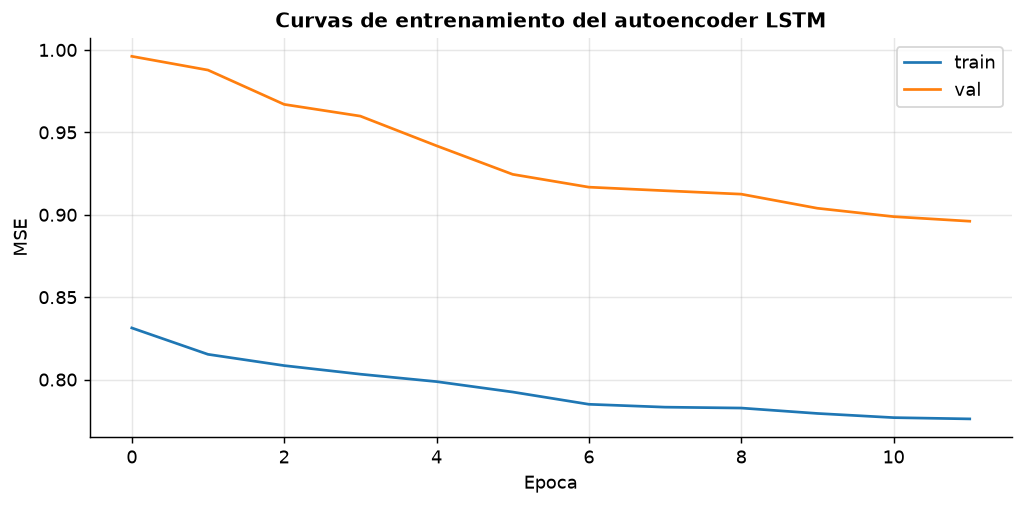
\includegraphics[width=0.72\textwidth]{../notebook/figures/training_curves.png}
\caption{Curvas de entrenamiento del autoencoder LSTM (train vs
validacion, MSE por epoca).}
\label{fig:training}
\end{figure}

\subsection{Distribucion del reconstruction error}

La figura~\ref{fig:distribucion} muestra la distribucion del error
para ventanas normales y con falla en el bloque de test, junto con
el umbral conformal y la curva precision-recall.

\begin{figure}[ht]
\centering
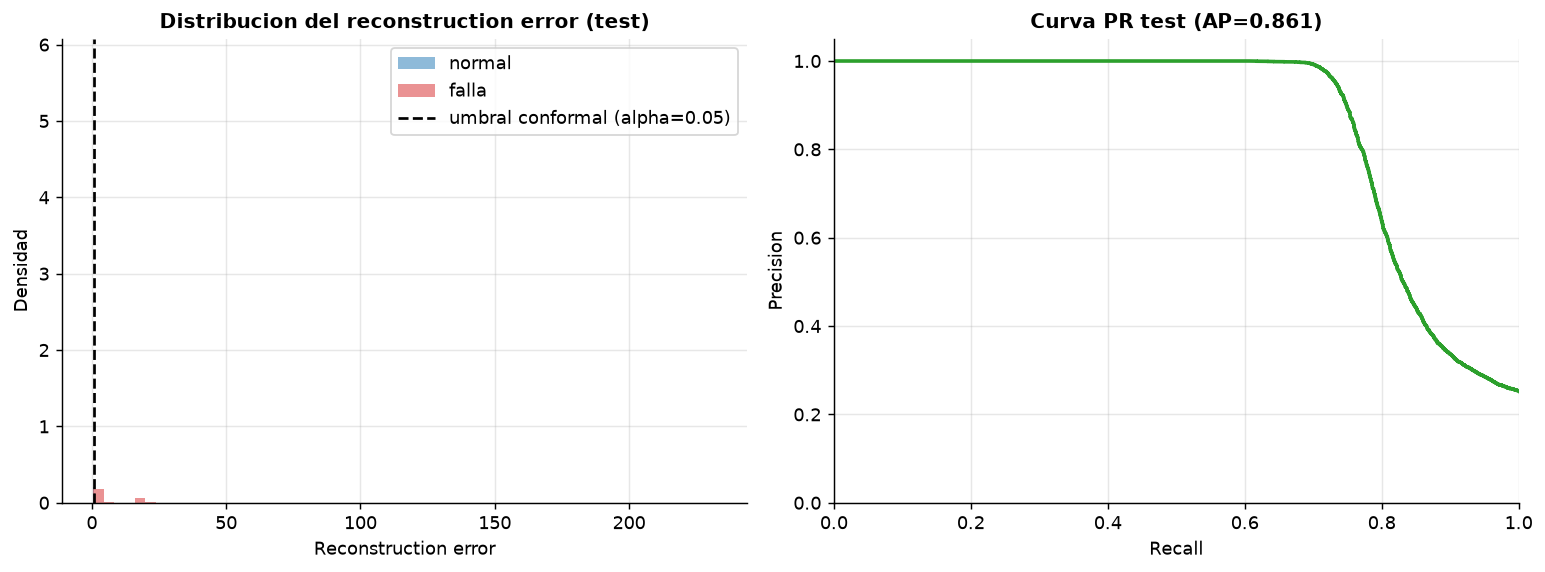
\includegraphics[width=0.95\textwidth]{../notebook/figures/conformal_diagnostics.png}
\caption{Diagnosticos conformal sobre el bloque de test:
distribucion del reconstruction error por clase y curva
precision-recall.}
\label{fig:distribucion}
\end{figure}

En regimen normal el error se concentra cerca de 1; bajo fallas
fuertes (cortocircuito, sobretension) supera 200. El solapamiento
que queda en la cola derecha corresponde a fallas lentas (F4,
F7): su firma crece de forma gradual y las primeras ventanas del
evento aun parecen normales. Ese solapamiento, y no la capacidad
del modelo, fija el techo de recall.

\subsection{Convergencia del aprendizaje federado}

La figura~\ref{fig:fedavg} compara FedAvg con el baseline
centralizado. La loss global del modelo federado baja de 3.826 a
3.724 en 4 rondas (119 s de CPU), y en deteccion el federado no
cede frente al centralizado: TPR $80.5\%$ vs $76.3\%$, AUC 0.906
vs 0.878.

\begin{figure}[ht]
\centering
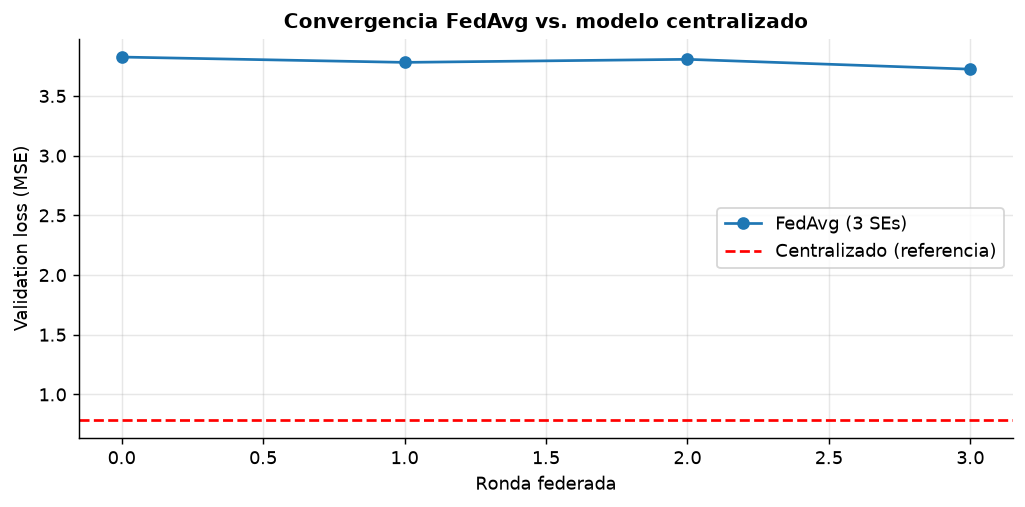
\includegraphics[width=0.72\textwidth]{../notebook/figures/federated_convergence.png}
\caption{Convergencia de FedAvg (3 SEs) vs modelo centralizado.}
\label{fig:fedavg}
\end{figure}

La lectura correcta no es que ``federar mejora la deteccion'':
el baseline centralizado entrena 6 epocas contra 4 rondas x 1
epoca local mas estadistica de 3 SEs, por lo que la comparacion
no es de presupuesto igual. El punto operativo relevante es otro:
\textbf{federar no cede detectabilidad} en este prototipo, y
mueve 0 MB de datos crudos fuera de las subestaciones. Para el
caso regulatorio chileno (aislamiento OT, NERC CIP), esa
equivalencia con privacidad por diseno vale mas que una decima de
AUC en cualquiera de las dos direcciones.

\subsection{Analisis por tipo de falla}

Con 25 eventos en 2 dias y cobertura garantizada por bloque, el
patron por tipo de falla es consistente con el diseno del
catalogo:

\begin{itemize}[leftmargin=*,itemsep=2pt]
  \item Las fallas agudas (F1 cortocircuito, F3 sobretension)
        disparan el score dos ordenes de magnitud sobre $\hat{q}$:
        deteccion en la primera ventana, latencia 0 s.
  \item Las fallas lentas (F4 degradacion de aislamiento, F7
        falla de buje) arrancan dentro de la banda normal y salen
        de ella a medida que la rampa crece: concentran casi todo
        el falso negativo del test.
  \item F8 (evento climatico) tiene la firma multivariable mas
        robusta (V, f, corrientes simultaneas), lo que valida el
        caso de uso post-frontal.
  \item F5 (perdida de comunicacion PMU) es estructuralmente
        invisible para un detector de residuos: la frecuencia
        congelada produce residuo $\approx 0$. Requiere un
        detector complementario de staleness (varianza nula,
        edad del dato), fuera del alcance de este prototipo.
\end{itemize}

\subsection{Tiempo de ejecucion}

Medido en CPU estandar (sin GPU):

\begin{itemize}[leftmargin=*,itemsep=2pt]
  \item Generacion de datos (2 dias, 172\,800 muestras): $\approx 1.5$~s
  \item Calculo de residuos: $\approx 0.1$~s
  \item Autoencoder centralizado (12 epocas): $\approx 60$~s
  \item FedAvg (4 rondas x 3 SEs x 1 epoca local): $\approx 119$~s
  \item Total: $\approx 5$~min
\end{itemize}

La inferencia por ventana es de milisegundos, compatible con
monitoreo en linea a cadencia SCADA de 1 Hz.

\subsection{Visualizacion interactiva}

El dashboard asociado (\texttt{dashboard/}, D3.js sin backend)
muestra el pipeline en operacion continua y permite interactuar
con cada etapa:

\begin{itemize}[leftmargin=*,itemsep=2pt]
  \item \emph{KPIs en vivo}: tensiones, corriente total, P/Q,
        frecuencia, temperatura de devanado y THD con sparklines y
        limites operativos (0.93/1.07 pu, 49.5/50.5 Hz, 95~°C).
  \item \emph{Controles de stream}: pausa, velocidad 1x/4x/16x,
        reinicio e inyeccion manual de cualquiera de las 8 fallas
        del catalogo desde la barra de control.
  \item \emph{Topologia unifilar}: SVG animado con flujo de
        corriente, disyuntores, carga por trafo y marcado de
        falla por elemento; clic en un alimentador selecciona su
        corriente en el panel de senales.
  \item \emph{Series SCADA/PMU}: observado vs esperado por el
        gemelo, bandas de falla, lineas guia de limites y
        crosshair con tooltip sincronizado con el panel de
        deteccion.
  \item \emph{Deteccion conformal}: score de reconstruccion vs
        umbral $\hat{q}$, zonas de alerta y ranking de features
        que impulsan el score (explicabilidad de la alerta).
  \item \emph{Mapa de calor residual}: 22 features x 90 s en
        streaming; clic en una etiqueta selecciona esa feature en
        senales.
  \item \emph{Aprendizaje federado}: mapa FedAvg con estado por
        SE, convergencia de loss vs centralizado y ronda actual.
  \item \emph{Timeline de eventos}: 4 h de simulacion con todos
        los eventos programados e inyectados, marcas de
        deteccion y playhead.
\end{itemize}

\subsection{Sintesis}

\begin{enumerate}[leftmargin=*,itemsep=2pt]
  \item \textbf{FPR empirico} $4.86\% \le \alpha = 5\%$: la
        garantia conformal se cumple con calibracion solo-normal y
        correccion de muestra finita.
  \item \textbf{Recall} $76.3\%$ (centralizado) y $80.5\%$
        (federado), con latencia mediana de deteccion $0$ s.
  \item \textbf{Gap federado vs centralizado}: inexistente en este
        prototipo (el federado mide levemente mejor); la
        equivalencia con 0 MB de datos movidos es el resultado
        accionable.
  \item \textbf{Costo}: $\approx 5$ min de CPU para entrenar y
        calibrar todo el pipeline, apto para reentrenamiento
        periodico.
\end{enumerate}

El capitulo siguiente discute estos resultados a la luz del marco
regulatorio chileno y de la literatura comparable.
